\section{Correctness}
When we say that BPaxos is ``correct'', what do we mean? In this section, we'll
answer this question.

\subsection{Generalized Consensus}
In \cite{lamport2005generalized}, Lamport introduces \defword{generalized
consensus} as a formal way to reason about the correctness of consensus
protocols. A full exposition of generalized consensus requires us to define a
new algebraic structure called a command structure set, or CStruct for short.
For this discussion though, we'll skip the details and focus on two particular
instances of generalized consensus: generalized consensus on logs and
generalized consensus on command histories.

\newcommand{\Cmd}{\Sigma}
\newcommand{\prefixof}{\sqsubseteq}
First up, \defword{generalized consensus on logs}. Let $\Cmd$ be a set of
commands. A log $x \in \Cmd^*$ is simply a string of commands. We write $x
\prefixof y$ to denote that $x$ is a prefix of $y$. We say $z$ is an upper
bound of $x$ and $y$ if $x \prefixof z$ and $y \prefixof z$. A log consensus
protocol (e.g., MultiPaxos, Raft) involves a set of clients that propose
commands and a set of learners that learn the state of the log over time. We
say such a protocol implements generalized consensus on logs if it satisfies
the following properties:
\begin{itemize}
  \item \textbf{Nontriviality:}
    At every point in time, the log $x$ learned by a learner can only contain
    commands proposed by a client.

  \item \textbf{Stability:}
    If a learner learns log $x$ at one point in time and log $y$ at a later
    point in time, then $x \prefixof y$. That is, a learner's log only grows
    over time.

  \item \textbf{Consistency:}
    For any two logs $x$ and $y$ learned by two different learners, there
    exists some upper bound of $x$ and $y$. That is, at any point in time two
    logs may not necessarily be equal, but they can be extended to be equal.

  \item \textbf{Liveness:}
    If a command is proposed, it eventually appears in a learned log.
\end{itemize}

\newcommand{\conflict}{\sim}
Next up, \defword{generalized consensus on command histories}. First, we
introduce \defword{Mazurkiewicz traces}~\cite{mazurkiewicz1986trace}. Again
consider a set $\Cmd$ of commands. Also consider a symmetric conflict relation
$\conflict$ over $\Cmd$. We say two commands $a, b \in \Cmd$ conflict if $a
\conflict b$. Consider two strings $x, y \in \Cmd^*$. We say $x \approx y$ if
there exists $u, v \in \Sigma^*$ and non-conflicting commands $a, b \in \Sigma$
such that $x = uabv$ and $y=ubav$. That is, $x \approx y$ if $y$ can be derived
from $x$ by swapping a single pair of adjacent non-conflicting commands. Let
$\equiv$ be the symmetric, transitive, reflexive closure of $\approx$. We say
two strings are equivalent if $x \equiv y$. The set of Mazurkiewicz traces with
respect to $\Cmd$ and $\conflict$ is the quotient $\Cmd/\equiv$.

More informally, a Mazurkiewicz trace is a string of commands, except that we
are allowed to repeatedly replace adjacent non-conflicting commands. For
example, letting $\Cmd = \set{a, b, c}$ with $a \conflict b$ and $a \conflict
c$, then
\[
  abca \equiv acba
\]
so the strings $abca$ and $acba$ represent the same Mazurkiewicz trace. Note
that Lamport calls Mazurkiewicz traces command
histories~\cite{lamport2005generalized}.

Mazurkiewicz traces are isomorphic to dependency graphs. A \defword{dependency
graph} $G = (V, E, \phi)$ is an acyclic directed graph $(V, E)$ with a function
$\phi: V \to \Cmd$ that labels each vertex with a command. The dependency graph
corresponding to Mazurkiewicz trace $a_1 a_2 \ldots a_n$ has $n$ vertices
labelled $a_1, \ldots, a_n$. The vertex labelled $a_i$ has an edge to every
vertex labelled $a_j$ where $j < i$ and $a_i \conflict a_j$. Conversely, The
Mazurkiewicz trace corresponding to a dependency graph can be formed by
topologically sorting the graph. Considering the example above, the trace
$abca$ has the following dependency graph:
\begin{center}
  \tikzstyle{vert}=[draw, thick]
  \tikzstyle{dep}=[-latex, thick]
  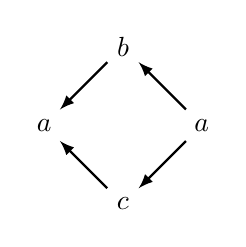
\begin{tikzpicture}
    \node (a0) at (0, 0) {$a$};
    \node (b) at (1, 1) {$b$};
    \node (c) at (1, -1) {$c$};
    \node (a1) at (2, 0) {$a$};
    \draw[dep] (b) to (a0);
    \draw[dep] (c) to (a0);
    \draw[dep] (a1) to (b);
    \draw[dep] (a1) to (c);
  \end{tikzpicture}
\end{center}

We write $x \prefixof y$ to denote that trace $x$ is a prefix of trace $y$.  We
say $z$ is an upper bound of $x$ and $y$ if $x \prefixof z$ and $y \prefixof
z$. A trace consensus protocol (e.g., EPaxos, BPaxos, Caesar) involves a set of
clients that propose commands and a set of learners that learn the state of the
trace over time. We say such a protocol implements generalized consensus on
traces (or command histories) if it satisfies the following properties:
\begin{itemize}
  \item \textbf{Nontriviality:}
    At every point in time, the trace $x$ learned by a learner can only contain
    commands proposed by a client.

  \item \textbf{Stability:}
    If a learner learns trace $x$ at one point in time and trace $y$ at a later
    point in time, then $x \prefixof y$. That is, a learner's trace only grows
    over time.

  \item \textbf{Consistency:}
    For any two logs $x$ and $y$ learned by two different learners, there
    exists some upper bound of $x$ and $y$. That is, at any point in time two
    logs may not necessarily be equal, but they can be extended to be equal.

  \item \textbf{Liveness:}
    If a command is proposed, it eventually appears in a learned trace.
\end{itemize}

Note that there really isn't any difference between generalized consensus on
logs and generalized consensus on traces. Alternatively, we can write $x
\prefixof y$ to denote that dependency graph $x$ is a prefix of dependency
graph $y$, and we can say $z$ is an upper bound of $x$ and $y$ if $x \prefixof
z$ and $y \prefixof z$. Then, we can define generalized consensus on dependency
graphs exactly as we did for traces.

\subsection{EPaxos Correctness Criteria}
Since Lamport introduced generalized consensus, some papers have adopted it as
the one true definition of consensus. For example,
Caesar~\cite{arun2017speeding} uses it, and we use it too. However, EPaxos
notably does not use it. Instead, they define their own correctness criteria
with definitions of nontrivialty, stability, consistency, execution
consistency, execution linearizability, and liveness. The most interesting is
execution consistency which is defined as ``If two interfering commands
$\gamma$ and $\delta$ are successfully committed (by any replicas) they will be
executed in the same order by every replica''.

This definition is not perfect. First, commands can be executed multiple times,
so we need some additional mechanism to disambiguate repeated commands. For
example, if a replica executes $\gamma$ then $\delta$ then $\gamma$ again, did
it execute $\gamma$ before $\delta$ or after? Second, execution consistency is
defined with a sense of liveness in it. It says commands ``will be executed''.
It's preferable to separate out liveness. Third, it's not obvious whether
EPaxos' correctness criteria are equivalent to those of generalized consensus.
Ideally, we wouldn't need a new set of correctness criteria for every new
protocol.

Still, EPaxos' definitions are \emph{much} simpler to digest that a full blown
description of generalized consensus. The EPaxos paper doesn't have to define
traces or dependency graphs, and it doesn't have to discuss prefixing or upper
bounds. It gets to the heart of the matter: conflicting commands should be
executed in the same order on all replicas.

\subsection{Reconciling Generalized Consensus and EPaxos}
In this section, we show that EPaxos' correctness criteria are easy to
formalize and that they are in fact equivalent to those of generalized
consensus on traces. This result lets us think about the correctness of EPaxos
and BPaxos either through the lens of forming dependency graphs or through the
lens of ensuring that conflicting commands are ordered the same across all
replicas.

First, we formalize the notion that one replica executes command $a$ before
command $b$. EPaxos and BPaxos replicas sequentially execute commands. These
commands form a trace $a_1, \ldots, a_n \in \Cmd^*$. The trace may contain
duplicates but fortunately, every command is chosen in a unique instance. Thus,
we can essentially think of commands as unique, where command $a$ chosen in
instance $I$ is different from command $a$ chosen in instance $J$.

Let $x \in \Cmd^*$ be such a trace. Let $a$ and $b$ be conflicting commands. We
say $a$ happens before $b$ in $x$, denoted $a < b$ in $x$, if one of the
following things is true:
\begin{itemize}
  \item
    $a, b \in x$ and $a$ precedes $b$ in $x$. Note that if $a$ and $b$ did not
    conflict, the notion of $a$ preceding $b$ would be ill-defined since a
    trace can re-order non-conflicting commands.

  \item
    $a \in x$ and $b \notin x$.
\end{itemize}
We say $a$ could happen before $b$ in $x$, denoted $x <_? b$ in $x$, if $a < b$
in $x$ or $a, b \notin x$.

Now, we can define EPaxos' correctness criteria the same as generalized
consensus on traces, except we'll define consistency as follows. For any two
traces $x$ and $y$ executed by two replicas, and for any two conflicting
commands $a$ and $b$, if $a < b$ in $x$ then $a <_? b$ in $y$.

TODO: Differentiating between $<$ and $<_?$ is a bit subtle. Work that out.

TODO: Prove that EPaxos consistency implies Generalized Consensus consistency.
- Long case analysis.

TODO: Prove that Generalized Consensus consistency implies EPaxos consistency.
- Prove that if $a < b$ in $x$, then $a < b$ in all prefixes of $x$.
- Case analysis.

% Well, defining the
% correctness of a state machine replication protocol like BPaxos turns out to be
% more complex that it may seem.
%
% Generalized
% Paxos~\cite{lamport2005generalized} formalizes \defword{generalized consensus}
% quite nicely, but it's pretty complicated. EPaxos defines its own form of
% correctness, but it's a tiny bit informal. Caesar~\cite{arun2017speeding}
% defines correctness using generalized consensus, but again, this is a little
% too complicated.
%
% Ideally, we'd like to define a very intuitive correctness criterion and prove
% that it is equivalent to generalized consensus. Here's an attempt at that.
%
% Let $\Sigma$ be a set of commands. Let $\Sigma!$ be the strings over $\Sigma$
% with no repeated commands. Let $x = x_1 \ldots x_n \in \Sigma!$. We say $a < b$
% in $x$ if (a) $a$ and $b$ both appear in $x$ and $a$ precedes $x$, or (b) $a$
% appears in $x$ but not $b$, or (c) neither appears in $x$. Consider two strings
% $x, y$ such that $a < b$ in $x$ if and only if $a < b$ in $y$. We want to prove
% that $x$ and $y$ are compatible. That is, there exists strings $w_x$ and $w_y$
% such that $x w_x \equiv y w_y$. If this is true, then the informal statement
% ``replicas execute conflicting commands in the same order'' is enough to
% maintain generalized consensus.
%
% The proof is likely going to be tricky. Reasoning about the equivalence of
% commands is always tricky. I think $w_x = y - x$ and $w_y = x - y$, but we'll
% have to see.
%
% Proof idea:
% In the Generalized Paxos paper, they say two histories are equivalent if they
% are permutations that preserve conflicting command ordering. If this is true,
% then I think we can prove our theorem easily. Append $(y-x) to x$ and $(x-y) to
% y$. They are permutations. Then, look at a conflicting pair of commands $a, b$
% in $x(y-x)$. Do a case analysis on where $a$ and $b$ appear. $a,b$ both in $x$;
% $a$ in $x$, $b$ in $(y-x)$, $a,b$ both in $(y-x)$. In all cases, we'll see that
Defining % $y(x-y)$ has them in the same order. Thus, the two strings are equivalent.
